\section{\ApproachName}
%! overview
\colorbox{text-highlight}{TO DO}

\subsection{Graph Wrangling}
% 从表格型数据创建图数据时,最重要的就是建立节点之间的关系。
% 观众从节点链接图中所能获知的信息仅仅是某两个节点之间存在联系,但却不了解联系的内在含义。
% 一些论文已经对可能建立链接的情况进行了定义,
Several techniques~\cite{DBLP:journals/ivs/LiuNS14, DBLP:journals/ivs/HeerP14, DBLP:journals/tvcg/SrinivasanPEB18} about graph wrangling identify link construction as the crucial process and propose several linking conditions.
Ploceus~\cite{DBLP:journals/ivs/LiuNS14} and Orion~\cite{DBLP:journals/ivs/HeerP14} infer potential linking conditions by first constructing a linking graph and then searching valid linking paths. They are aimed at constructing links among multiple data tables by analyzing primary keys and foreign keys.
Graphiti~\cite{DBLP:journals/tvcg/SrinivasanPEB18} identifies potential linking conditions of a homogeneous graph by comparing different attributes.
% 如果多个表合并成一个表,前两者总结的条件可以被Graphiti提出的规则所覆盖
Because multiple tables can be merged into one data table with primary keys and foreign keys, Graphiti can cover the linking conditions identifying rules proposed by Ploceus and Orion. %? 这里mayby要用一张图解释一下
We reorganize the conditions proposed by these techniques into four categories:
\begin{compactenum}[\textbf{Cond.} 1.]
    \item Two nodes share a same value of a same attribute, e.g., linking two movies is published in the same year.
    \item Two nodes share at least one same common value of a same list attribute, e.g., linking two movies with one or more same actors.
    \item Two nodes share significantly close value of a same attribute where the significance is defined by the normalized difference.
    \item Two nodes share two values in the same bin of a same attribute where the bins are defined as quartiles.
\end{compactenum}
Hear, we regard sharing same topics of textual attributes as same as sharing same values of list attributes (Condition 2), because topics are often presented as a list attribute.

% 我们尝试从它们的反方向进行思考,也就是,当我们获取到了所有的链接的时候,推测这些链接是如何被构建的
Those works infer the potential linking conditions before all links are constructed. 
Whereas, our method runs in the opposite direction where all links have been constructed already.
% 针对某一条链接,可能有不止一种构建条件,我们取所有链接的构建条件的交集作为整个graph的构建条件。
We traverse all links to detect potential conditions for each link.
The intersection of all links' conditions are regarded as the entire graph's linking condition.

% 为了能够将这些condition填充到文本模板中,我们对condition的输出进行了formalize
At last, we formalize the condition as three aspects, and textualize the linking condition of the graph by filling templates. 
One condition can be defined as:
\begin{equation}
    \text{linking condition} := ( type, attribute, value )
\end{equation}
Four templates corresponds to four conditions according the $type$:

\begin{compactenum}[\textbf{Cond.} 1.]
    \item ``Two nodes are connected if their attributes $[{attribute}]$ are with a same value$\{: [{value}]?\}$''.
    \item ``Two nodes are connected if their attributes $[{attribute}]$ share an intersection$\{: [{value}]?\}$''.
    \item ``Two nodes are connected if their attributes $[{attribute}]$ are close, maybe with a difference less than $[{value}]$''.
    \item ``Two nodes are connected if their attributes $[{attribute}]$ are within the same bin$\{: [{value}]?\}$''.
\end{compactenum}

Where $[{attribute}]$ is the name of the attribute, $[{value}]$ is the value of the attribute, and $\{?\}$ means the included part is optional. 
For example, for Condition 2, two movies are connected because they share same actors Alice and Bob. 
The condition is represented as: $(\text{``Condition 2''}, \text{``actors''}, [\text{``Alice''}, \text{``Bob''}])$. 
Its corresponding statement is: ``Two nodes are connected if their attributes ``actors'' share an intersection: [``Alice'', ``Bob'']''. 
And there is an implication relation between conditions.
Some conditions are stronger than others.
For example, the condition $(\text{``Condition 2''}, \text{``actors''}, [\text{``Alice''}, \text{``Bob''}])$ is stronger than $(\text{``Condition 2''}, \text{``actors''}, [\text{``Alice''}])$ and $(\text{``Condition 2''}, \text{``actors''}, [arbitrary\text{ }value])$.
All the three conditions are regarded as individual conditions.

If a linking condition exists on both nodes with links and nodes without any link, it is regarded as a false condition and should be filtered out.
We describe our filtering strategy in~\ref{alg:conditions}.
After that, conditions are sorted, so that the highest ranked condition will be regard as the most possible condition.
First, all conditions are sorted by their frequency.
% 相同频率的条件,如果他们的type和attribute相同,那么根据
If two conditions with the same frequency have the same $type$ and $attribute$, they can be compared by their degree.
More stronger conditions are ranked higher than others.


% 一条边可能包含多个条件,不同边的条件之间可能有交集,可能没有交集。
% 我们需要一个策略来得到一个关于节点之间如何构建出关系的结论。
%! 解释一下算法
% 首先,对于所有没有边的节点对,找出所有可能的构建条件。
% 其次,对于某条边,它的构建条件和上述的构建条件之间找出差集。
% 最后,所有边的条件的合集属于边的构建条件;其中 频率最高的将被拿出来。



\begin{algorithm}[!t]
    \renewcommand\arraystretch{1.2}
    \caption{ Conditions filtering }
    \label{alg:conditions}
    \begin{algorithmic}[1]
        \Require
            $G=(V=\{v_1, v_2, ..., v_n\}, E=\{e_1, e_2, ..., e_n\})$: a graph;
        \Ensure
            $C$: conditions
        \State Init conditions $C=\varnothing$, false conditions $FC=\varnothing$
        \For {each node pair $(v_i, v_j)$}
            \If {$(v_i, v_j)$ is not a link}
                \State $C_{tmp} \gets$ all conditions that can link $(v_i, v_j)$
                \State merge $FC$ with $C_{tmp}$
            \EndIf
        \EndFor
        \For {each link $e_i$}
            \State $C_{tmp} \gets$ all conditions that can construct link $e_i$
            \For {each condition $c$ in $C_{tmp}$}
                \If {$c$ in $FC$}
                    \State remove $c$ from $C_{tmp}$
                \EndIf
            \EndFor
            \State merge $C$ with $C_{tmp}$
        \EndFor
        \State \Return $C$
    \end{algorithmic}
\end{algorithm}


\subsection{Visual Encoding}
% 为了在节点链接图中展示节点、链接的属性,常常将这些属性编码为节点/链接的视觉通道。
To visualize attributes of nodes and links in node-link diagrams, creators often encode them with visual channels on nodes and links.
For example, in Figure~\ref{fig:VisualEncodings} (a), a node contains a categorical attribute (\textit{x}) and two numerical attributes (\textit{y} and \textit{z}), we encode two numerical attributes with two rectangles' height and encode the categorical attribute with two rectangles' fill color and the background circle's stroke color.
We denote graphical elements (e.g., \texttt{<circle>}, \texttt{<rect>}, \texttt{<ellipse>}, etc.) in node-link diagrams as \textit{visual primitives} and their style attributes such as \texttt{cx}, \texttt{cy}, \texttt{width}, and \texttt{height} are denoted as \textit{visual channels}.
Nodes and links contained in the underlying graph are denoted as \textit{data entities} and each data entity consists of several \textit{attributes}.


\begin{figure}
    \centering
    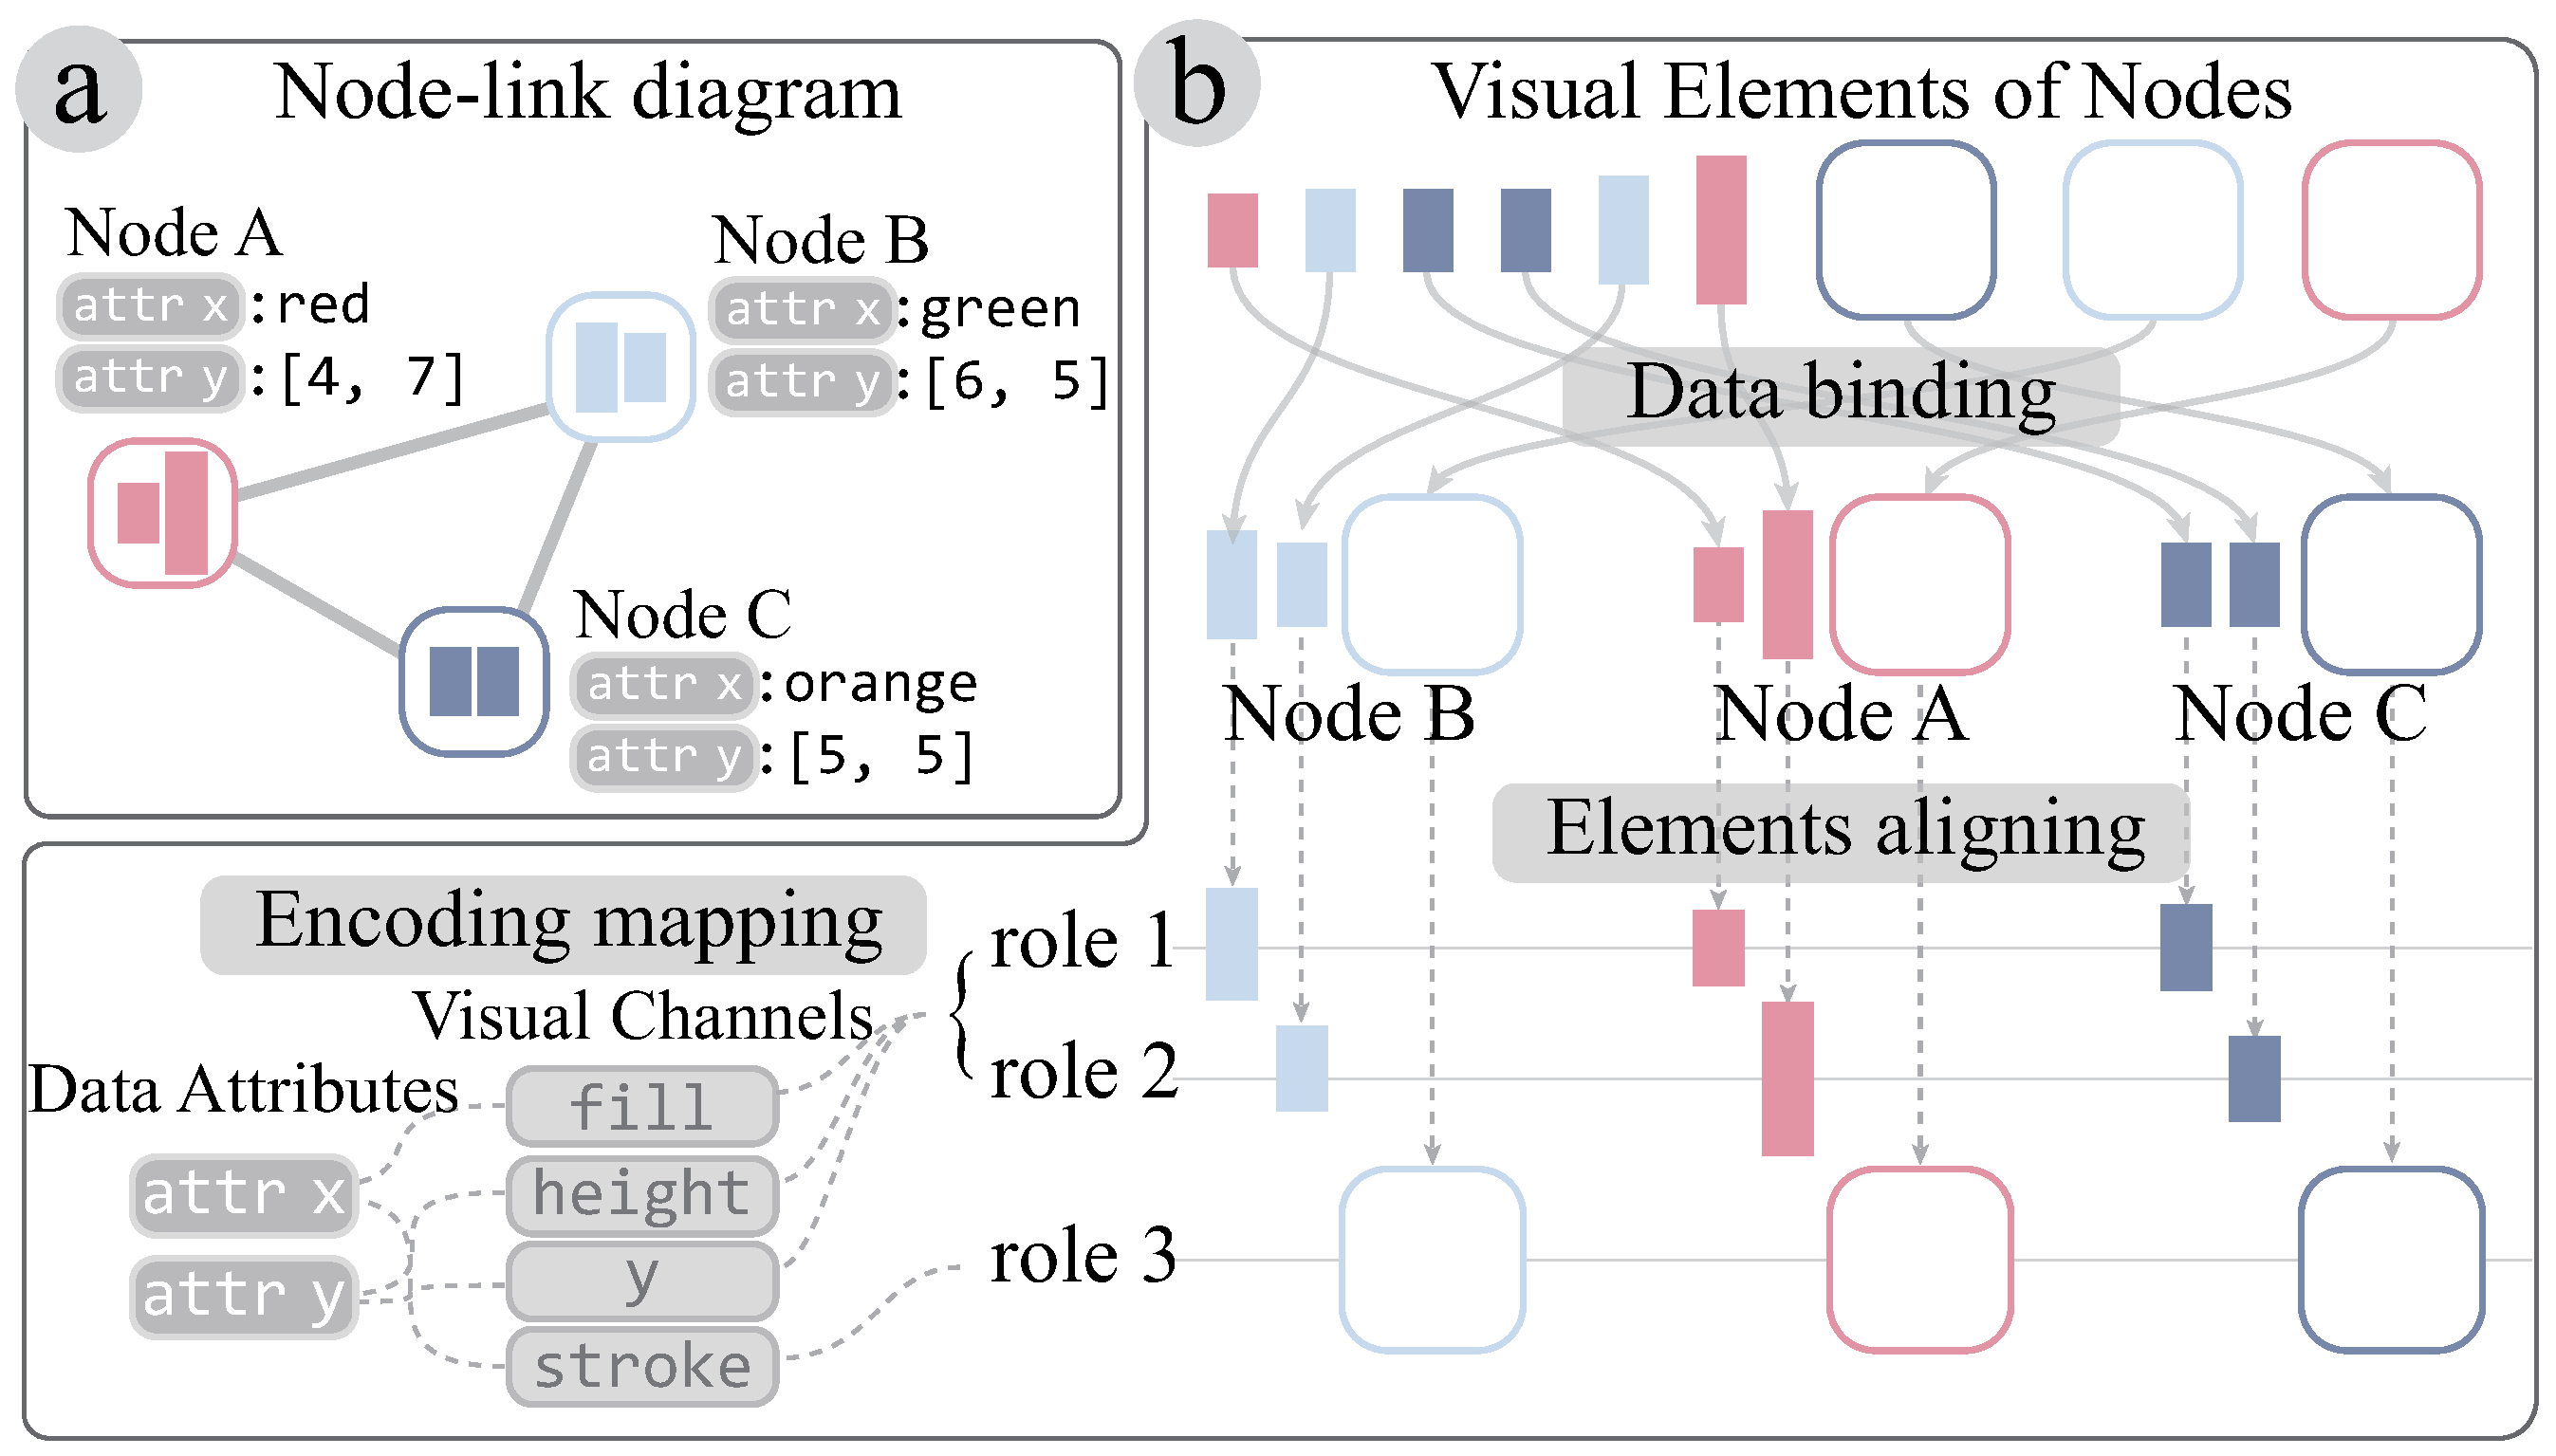
\includegraphics[width=1\columnwidth]{figures/VisualEncodings.eps}
    \caption{(a) A node-link diagram shows a visual encoding example. (b) The main target of our visual encoding detecting technique is to bind data entities (nodes and links) to visual primitives (SVG elements) and map data attributes to primitives' visual channels.}
    \label{fig:VisualEncodings}
\end{figure}

% 我们的工作通过分析源代码,从中提取数据实体()是如何被编码为视觉通道的()
To describe visual encodings of a node-link diagram, how attributes of data entities (nodes and links) are encoded with visual channels (style attributes of SVG elements) should be determined.
% xxxx 等人的工作为我们提供了一个良好的思路,但他们的工作存在一些限制
A tool proposed by Harper and Agrawala~\cite{DBLP:conf/uist/HarperA14} provides a creative perspective for detecting visual mappings.
Although their tool can be extended to support simple node-link diagrams (where each data entity is encoded into only one primitive), it has several limitations:
\begin{compactenum}

% 1. 其需要创作者使用d3的数据绑定,才能发挥__data__的作用;使用其他工具,或者未将数据绑定到元素上时则无法使用该方法;
\item The data binding feature of D3 is required within the tool such that the ``\textit{\_\_data\_\_}'' attribute of visual primitives can be acquired by it. 
It cannot deal with SVG-format visualizations created by other tools or without data bound to visual primitives.

% 2. 其只能检验属性和视觉通道之间是否存在线性映射或者类别性映射。
\item Only the linear mapping and categorical mapping are supported, it cannot maintain situations where visual mappings are complex.

\end{compactenum}

% 我们针对节点链接图的场景,提出了一个数据绑定的策略,通过不断调整输入的数据,检查输出的变化,从而获取数据到svg元素之间的映射关系以及属性到视觉通道之间的映射方式,以解决以上两个问题。
For node-link diagrams, we introduce a new technique to solve such limitations.
The main idea of our technique is regarding the source code as a black box model.
Our technique obtains mappings between data entities and visual primitives by detecting changes of the output SVG after modifying the input graph data.
It overcomes the limitations by binding data to visual primitives and detecting visual mappings between data attributes and visual channels (Figure~\ref{fig:VisualEncoding} (b)).
% It can bind data to visual primitives and detect visual mappings between data attributes and visual channels to overcome the limitations.


% 在开始介绍算法之前,我们先列出我们对于通用情况的几点假设
% 1. 映射方式只跟数据分布相关(比如最大值最小值),当不改变数据的分布时,映射方式也不会改变;
% 2. 每个node都只会影响它自己相关的视觉元素的视觉编码,不会影响其他node;同样link也是(但节点可能会影响边)
% Before we introduce the technique, we list several assumptions that our technique requires:
% \begin{compactenum}
% \item Only the distribution of the data can influence the visual mapping scheme (e.g., the maximum value and the minimum value). 
% Only swapping two data entities will not cause any change of the visual mapping scheme.

% \item Swapping two nodes will not influence SVG elements related to other nodes; and so do links.
% Note that this assumption does not assume that swapping nodes will not influence links.

% \item Every nodes share a same encoding scheme and every links also share a same encoding scheme.
% \end{compactenum}
% % 我们认为这些情况是很常见的,适用于很多情况。我们的 gallery 也证明了我们的技术可以适用于很多case。
% Our gallery in the case study ({\color{text-highlight}Section~\ref{}}) suggests these assumptions are general in many cases.

% 首先,我们将svg视作一个树结构,其通过最广搜索算法或者最深搜索算法可以生成一个数组,称为svg数组。该数组只包含会产生视觉特征的svg元素:圆...等
% We regard the output SVG as a tree and use the Depth-First Search algorithm to generate a primitives list. 

% 我们首先交换任意节点对的属性。
\textbf{Data binding} is first achieved.
To detect mappings between data entities and visual primitives, 
we modify attribute values of data entities and record corresponding visual primitive changes.
Mappings between the entity and the changed primitives are hence constructed.
However, modifying attributes deforms the attribute distribution, which may influence visual mappings, so that primitives related to other data entities may also change.
For example, modifying attributes may expand the data range and thus changes linear mappings defined by attribute ranges.
We prevent it by only swapping two entities rather than modifying it, such that no new data is introduced and the data distribution is preserved.
We take nodes for example.
Each node will be swapped with all the other nodes.
Primitives changed by each swapping correspond to two swapped nodes (Figure~\ref{fig:DataBinding} (b) and (c)).
For example, after swapping nodes B and C in Figure~\ref{fig:DataBinding} (b), primitives 1 to 4 are changed.
All these changed primitives correspond to nodes B and C, because only B and C are modified.
After swapping one node with all the other nodes, we construct mappings between the node and primitives which are changed more than once.
For example, after swapping nodes B with C and D in Figure~\ref{fig:DataBinding} (b) and (c), primitives 2 and 3 are changed twice, thus they correspond to node B.
After swapping all nodes, the entire node-primitive mappings are constructed (Figure~\ref{fig:DataBinding} (d)).
Mappings between Links with their primitives are constructed in the same.
Because swapping two nodes may influence their related links, nodes' related primitives can contain links' primitives,
we remove links' primitives from the node-primitive mappings.

Here, we only classify visual primitives into different data entities.



\textbf{Visual encoding} is then extracted by shuffling attribute values and detecting visual channel changes.
% 我们继续以节点为例。
We continue to take node as for example.
% 为了检验一个属性究竟被编码在了哪些视觉通道上,我们通过shuffle所有节点的某个属性,观察视觉通道发生的变化。
We map one attribute to its related visual channels by first shuffling the attribute of all nodes and then observing the changes of visual channels.
% 发生变化的视觉通道就和该属性相关,于是他们之间的映射关系就被构建好了。
Mappings are built between the attribute and those visual channels.
% 我们抽选了一些常用于编码信息的通道:比如....
% tagName是最特殊的一类,它直接能切换不同的primitives种类。
% 比如一个节点可能根据某个类别型属性被编码为圆形或者矩形。
% 而且,一个属性可能在该primitive表现为不同形状时,编码了不同的通道。
% 比如节点的某个数值型属性会用来表示size,在圆形的时候就是r,在矩形的时候就是width和height。
% 我们在描述的时候就应该将它们当做同一种primitives,因为他们的编码方案是一致的。
% 也就是说,我们应该根据编码方案对primitives进行分类~\ref{...}。
% 然而,我们难以


\begin{figure}
    \centering
    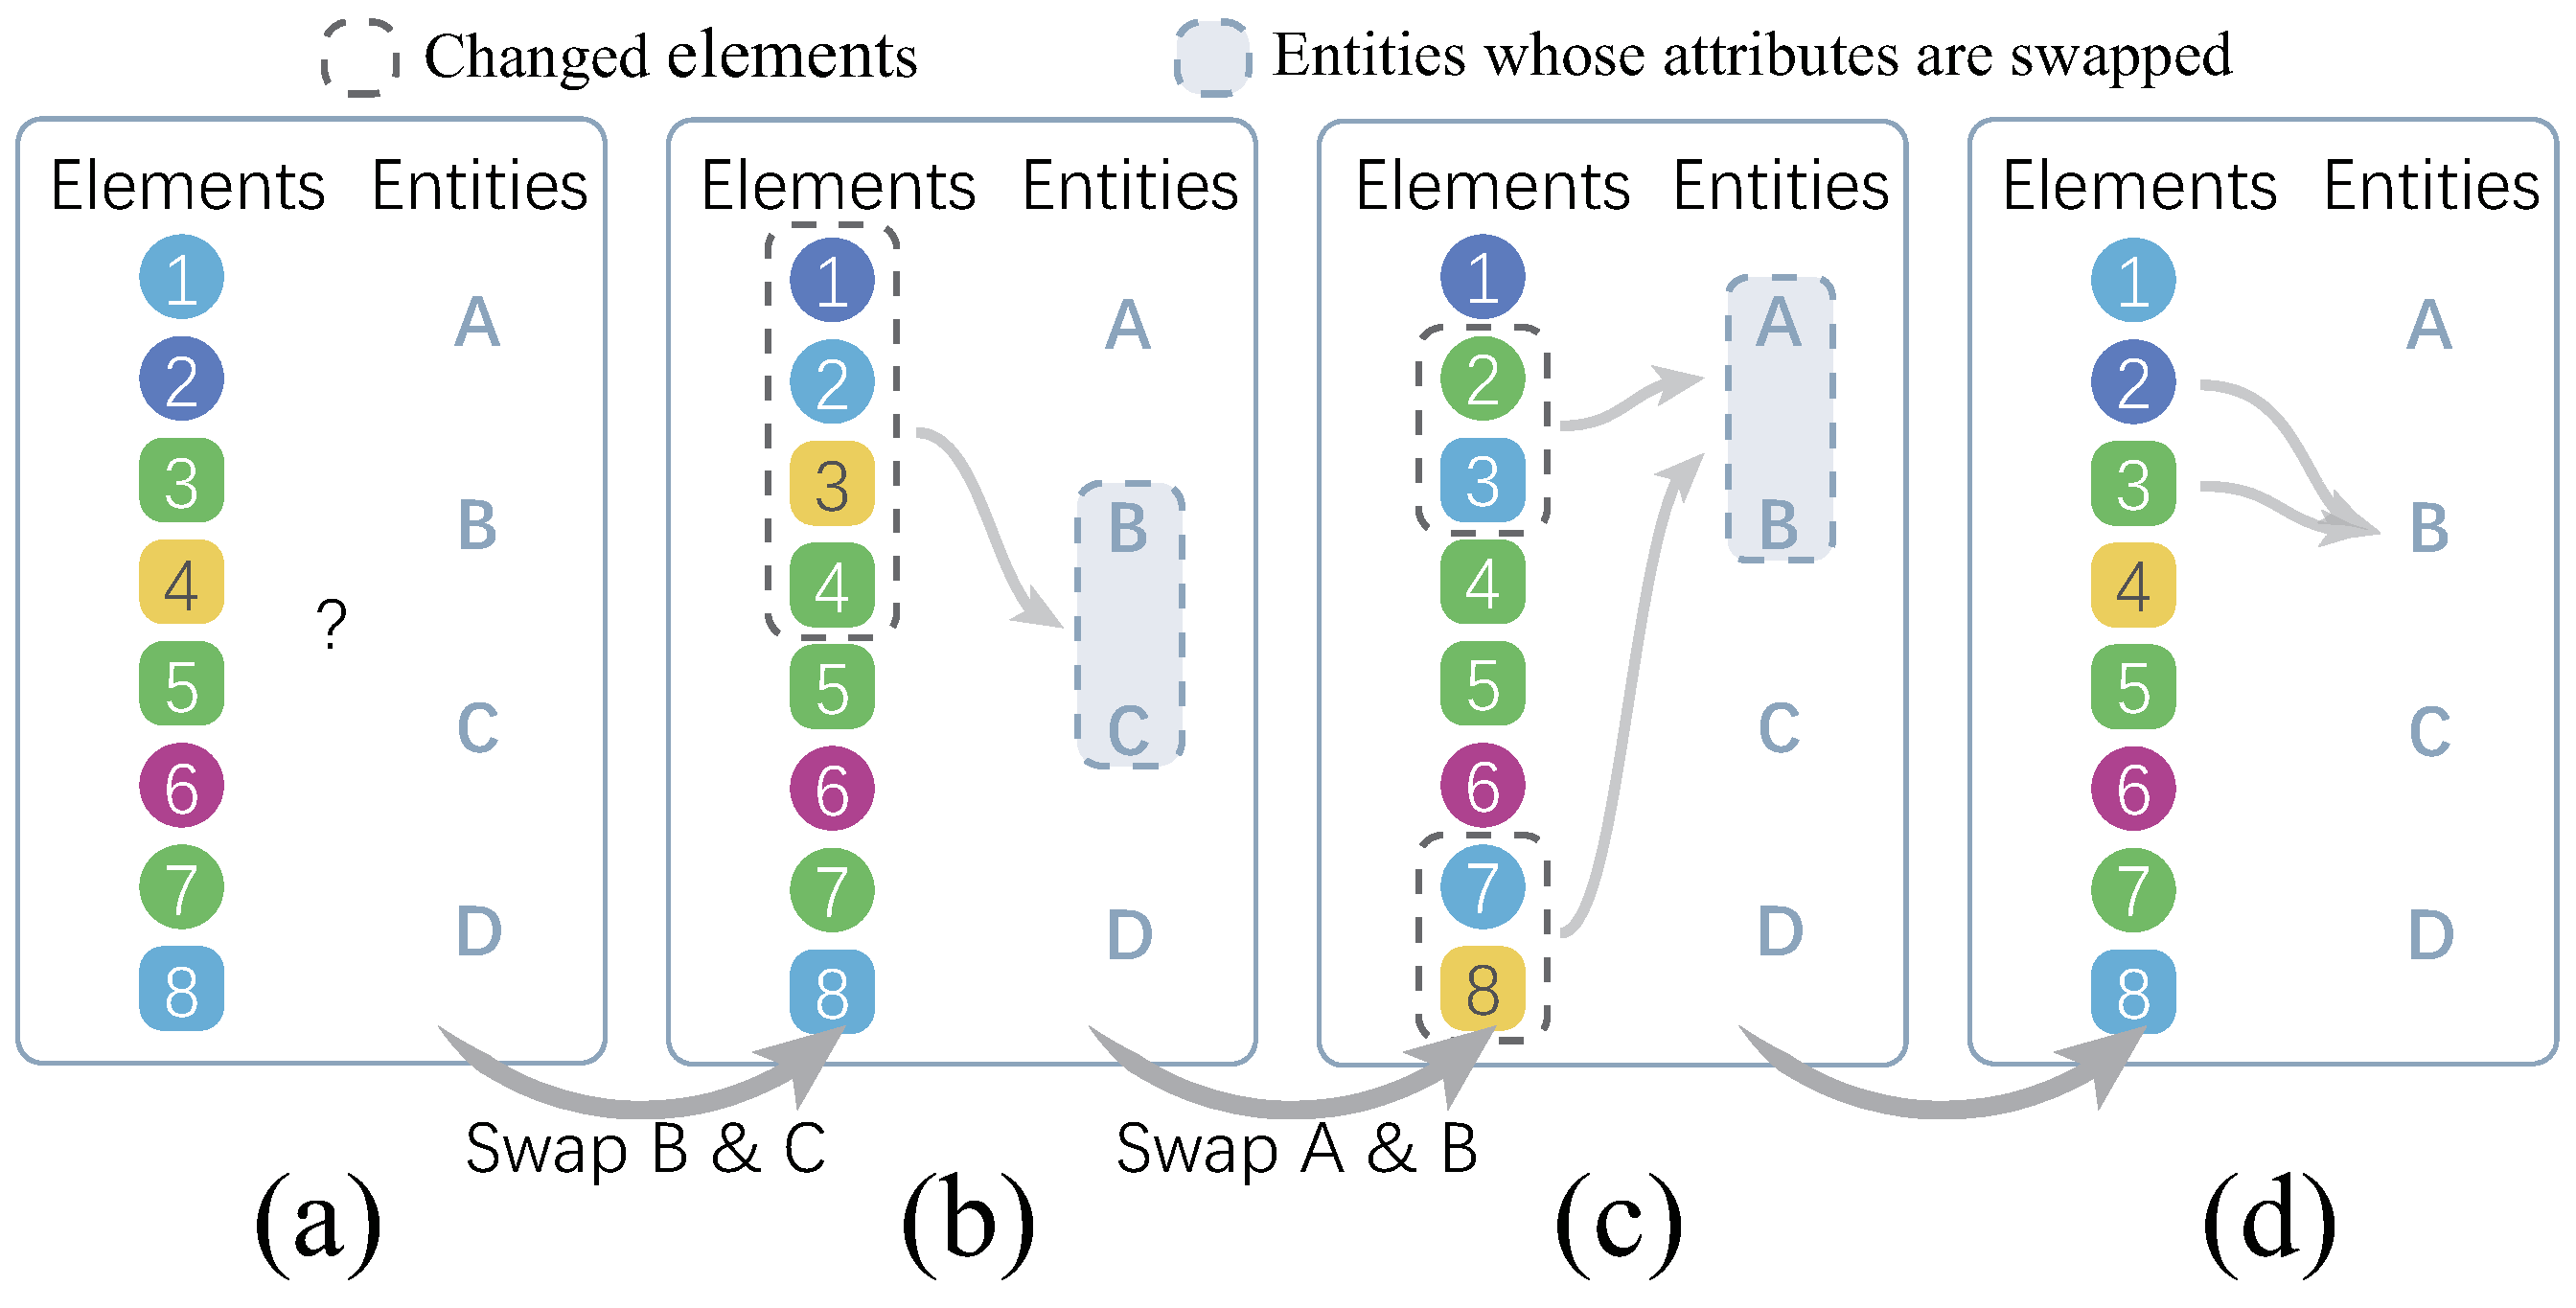
\includegraphics[width=1\columnwidth]{figures/DataBinding.eps}
    \caption{Data binding is achieved by swapping attributes of data entities. (a) Visual mappings between original visual primitives and data entities are unknown. (b) After swapping attributes of entities B and C, the appearance of primitives 1 to 4 is changed. Thus, entities B and C correspond to primitives 1 to 4. (c) After swapping attributes of entities A and B, the appearance of primitives 2, 3, 7, and 8 is changed. Thus, entities A and B correspond to these primitives. Primitives 2 and 3 are changed twice, we can map the entity B to primitives 2 and 3. (d) After swapping all nodes, the entire node-primitive mappings are constructed.}
    \label{fig:DataBinding}
\end{figure}


% 首先我们获取节点的所有属性(除唯一标识符id之外),遍历这些属性,对某个属性alpha:
% 我们通过调换两个节点(记作A和B,要求A和B的属性alpha不同)的属性alpha,记录svg数组中发生变化的项目(记作Set_{AB})
% 在保留A的情况下,将B换成其他存在alpha属性不同的节点不断重复,对所有记录下来的项目变化求交集,即为A节点对应的视觉元素;
% 在此过程中,我们还能获取到属性A能够改变的视觉通道。
% 然后对于所有属性求出来的节点A对应的视觉元素的集合求并集,即为节点A对应的视觉元素;
% 对所有的边进行相同的步骤,找出每条边所对应的视觉元素。
% 从节点所对应的视觉元素中,减去边所对应的视觉元素。
% 最终我们就可以将数据绑定到视觉元素上了。
% 其中还有一种特殊情况,也就是只存在一个节点和A节点的数据不同。那么我们可以先把A节点换成该节点的数据。那么只要有超过两个节点的图数据,我们都能为A节点找到两个跟它数据不一样的节点了。
% 该过程的时间复杂度为O(k_n*N^2+k_e*M^2)
% 该过程为饱和式检查,保证了准确性;我们可以通过只交换A节点和B、C节点后求交集后就终止检查来将时间复杂度降低到O(k_n*N+k_e*M),但会牺牲某些特殊情况下的准确性,比如.... 在实践过程中,我们可以通过调整参数x来平衡时间复杂度和精度之间的关系。

% 如果某个视觉通道,只有同时改变两个属性才能发生变化...这种情况就没法detect了


% 在上述的过程中,我们还获取到了数据属性是如何影响视觉通道的。
% 我们利用抽取的数据,来描述节点链接图的视觉编码方案:
% 1. 节点/链接的组成元素分别是什么?
% 2. 视觉通道的决定性因素(属性)是什么?
% 3. 视觉通道和其决定性因素的相关性如何?(正相关/负相关/类别相关..)

% 对于一个节点包含的多个视觉元素。我们对他们进行分组描述,分组的依据是视觉元素的编码方案是否一致。
% 同样的,如果不同的节点有不同的编码方案,我们也会对它们进行分组描述。


% 我们尝试从这几个方向增强该方法,并配合节点链接图的特性,帮助创作者更好的解释节点链接图中的编码方案。
% 我们发现,虽然 Deconstructing and Restyling D3 Visualizations 的方法只需要svg作为方法的输入,但它的svg是处于运行环境中的,也就是说,如果没有运行源代码,__data__属性也就没法绑定到对应的元素中。所以它隐式地依赖于可视化创作者的源代码。所以我们还可以使用其源代码用于分析。


%! 我们的方法的过程
% 我们对Deconstructing and Restyling D3 Visualizations进行了改进;主要从x方面进行:
% 作为该方法的补充,为了使数据绑定能够应用于非d3创建的代码,我们提出了一个检验方法,它将创建者创建的代码视作黑盒,通过修改输入的数据,检验输出的svg元素的变化来获取编码方案。
%? 这里假设了修改源数据,不会对代码造成影响,但实际上很多情况下,映射方式会根据数据本身进行更改,比如数据值的范围。可以放在discussion里面讨论一下。
% 下面的章节我们围绕着几个方面进行:
% 1. 如何为没有为没有进行数据绑定的svg,找到每个节点和链接对应的元素,以补充 Deconstructing and Restyling D3 Visualizations;
% 2. 新的视觉通道和属性之间的关联检验方式,防止出现多属性之间线性依赖以及复杂映射情形失效的情况;
% TODO下面都是围绕节点和链接展开,但我们的方法不仅仅能够解决节点链接图的可视化,也可以用用于其他类型的可视化形式。

%! 讲一下我们主要检测的基础视觉元素:

%! 1 首先对某个属性做出修改,但不修改数据分布,只调换数据顺序;查看哪个/些视觉通道发生了变化;找到那些不改变dom结构的属性(tagname和element数量);
%!  对嵌套结构(数组/对象)进行说明:没有关系,等详细说明映射方式的时候再决定;
%! 2 过滤掉会对svg element的tagName和数量产生影响的属性,交换A节点和B节点的其余数据,观察哪些svg的视觉通道发生了变化;然后恢复数据;再交换A节点和C节点的其余数据,观察通道变化;取两次的交集的svg element,它们绑定的数据就是A节点;


% 我们首先提出了对该方法的增强算法,使该方法能够泛化到更通用的场景下。
% 因为我们方法目的是为创作者提供自动创建节点链接图描述的技术,所以我们假设了创作者的创作源码可以输入到我们的方法中用于提取信息。
% 虽然xxx等人的方法没有假设源代码的存在,但实际上,运行环境下,想要获取到svg元素的__data__属性,必定有运行中的JavaScript程序在背后支持,所以该工作也隐含了javascript的源码存在的假设。


\subsection{Layout}

\subsection{Interview \& Iterative Design}

\subsection{Understanding Visual Clutter}